\documentclass[12pt,letterpaper]{article}
\usepackage[utf8]{inputenc}

\usepackage[spanish]{babel}
\usepackage{amsmath}
\usepackage{color}
\usepackage{algorithm}
\usepackage[noend]{algpseudocode}
\renewcommand{\algorithmicrequire}{\textbf{Entrada:}}
\renewcommand{\algorithmicensure}{\textbf{Salida:}}
\usepackage{subcaption}
\usepackage{amsfonts}
\usepackage{hyperref}
 \hypersetup{
     colorlinks=true,
     linkcolor=blue,
     filecolor=blue,
     citecolor = blue,      
     urlcolor=cyan,
     }
\usepackage{amssymb}
\usepackage{listings}

\usepackage{amsthm}
\newtheorem{theorem}{Teorema}

\usepackage{graphicx}
\usepackage[left=2cm,right=2cm,top=2cm,bottom=3.5cm]{geometry}
\setlength{\parskip}{3mm}
\title{\textsc{Práctica 5: \\ Método Monte-Carlo}}
\author{\textsc{Fabiola Vázquez}}

\setlength{\parindent}{0cm}
\renewcommand{\lstlistingname}{Código}
\floatname{algorithm}{Algoritmo}
\spanishdecimal{.}
\begin{document}
\maketitle

\hrule
\section{Introducción}
El objetivo de esta práctica \cite{elisapractica5} es aproximar el resultado de una integral utilizando el método Monte-Carlo, variando el tamaño de la muestra, al valor proporcionado por WolframAlpha \cite{wolfram}. El experimento se realiza con el software R versión 4.0.2 \cite{R} en un cuaderno de Jupyter \cite{jupyter}.

\section{Experimento}
Se quiere aproximar el resultado de la siguiente integral 
\begin{equation}
\int_3^7 \frac{dx}{\exp(x) + \exp(-x)}.
\end{equation}
Para ello se generan números pseudoaleatorios con distribución $g(x)=\frac{2}{\pi}f(x)$, donde $f(x)=\frac{1}{\exp(x) + \exp(-x)}$, haciendo uso de la función \texttt{r(AbscontDistribution(d = g)).} El código del experimento \cite{fabiola} está basado mayormente, en el código implementado por Schaeffer \cite{codigoelisapractica5}. 

Como se quiere comparar el valor de la integral obtenida mediante la simulación con el valor proporcionado por Wolfram (denotado como \texttt{wolfram}), la función \texttt{decimalesexactos}, descrita en el código \ref{lst:gc1}, nos regresa la cantidad de decimales en que son coinciden dichos valores.

En el experimento se varía el valor del parámetro \texttt{pedazo} de 1000 a 10000 en saltos de 1000, pero no se aproximaba tanto al valor de \texttt{wolfram}, por lo que se varía en otros rangos como de 50 a 500 y de 50000 a 95000, haciendo 50 réplicas con cada uno. El cuadro \ref{datos} muestra un fragmento de los datos recopilados en el experimento y la figura \ref{box1} muestra los gráficos de caja bigote de los valores de la integral obtenidos en el experimento. Como se puede apreciar en dicha figura, a mayor valor de \texttt{pedazo} más se aproxima al valor de \texttt{wolfram}.

En la figura \ref{box2} se muestran los decimales exactos obtenidos en las variaciones del tamaño de \texttt{pedazo}. Como se aprecia, entre mayor es el tamaño más decimales se aproximan al valor de \texttt{wolfram}. Aún cuando el tamaño de \texttt{pedazo} se varía en una gran número, no fue posible aproximarse al valor de \texttt{wolfram} a mas de cuatro decimales, y aumentar a un mayor valor no fue computacionalmente posible. 
 
\begin{lstlisting}[label=lst:gc1,caption=Función \texttt{decimalesexactos}., frame = single]
decimalesexactos <- function (x){
    for (i in 1:6){
        if (!(trunc(wolfram*10^i)==trunc(x*10^i))){
            return(i-1)
            break
        } 
    }
    return(6)
}
    
\end{lstlisting} 

\begin{table}
\centering
\caption{Fragmento de los datos obtenidos en el experimento}
\begin{tabular}{rrrr}
  \hline
 Corrida & Pedazo & Integral & Precisión decimal  \\ 
  \hline
1 & 1000 & 0.0488361 & 5 \\ 
  105 & 3000 & 0.0488884 & 4 \\ 
  210 & 5000 & 0.0488486 & 4 \\ 
  320 & 7000 & 0.0488275 & 4 \\ 
  400 & 8000 & 0.0487473 & 3 \\ 
  700 & 65000 & 0.0489142 & 3 \\ 
  900 & 85000 & 0.0488143 & 4 \\ 
   \hline
\end{tabular}
\label{datos}
\end{table}
 
\begin{figure}
	\centering
	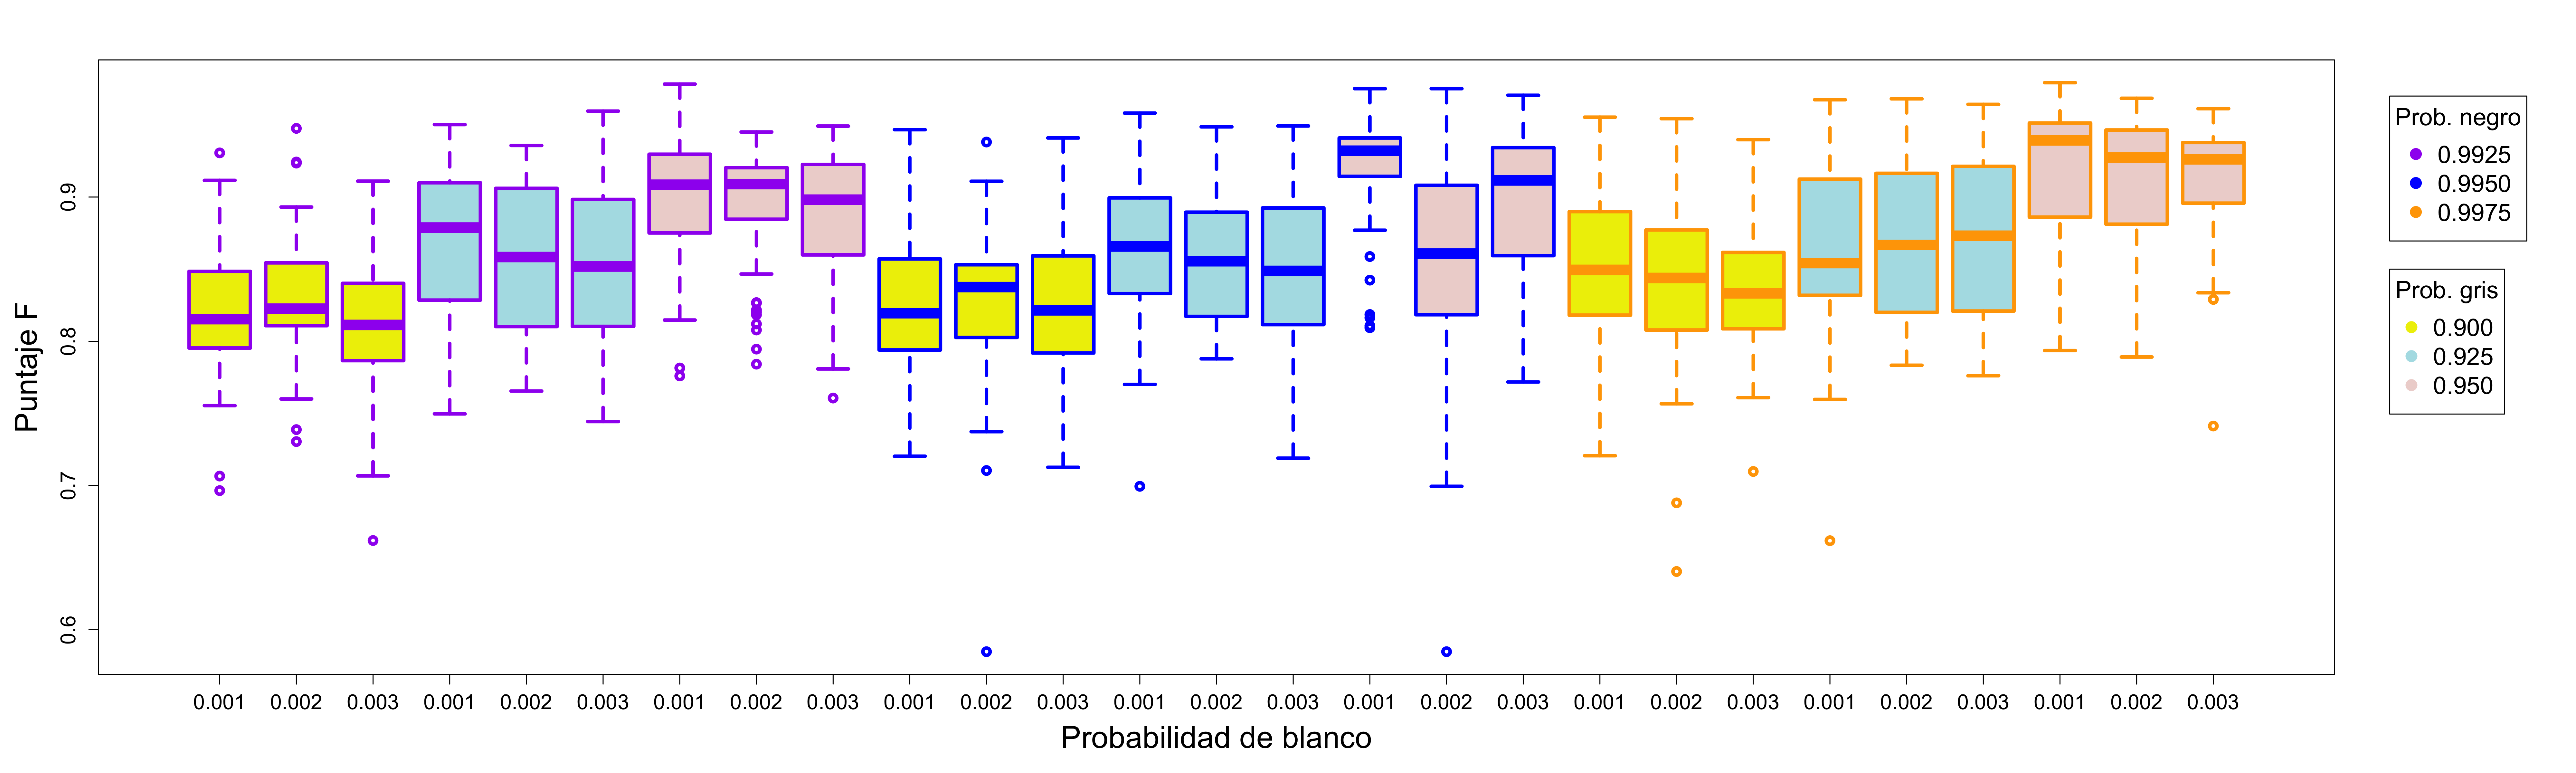
\includegraphics[width=\linewidth]{boxplot.png}
	\caption{Gráficas de caja bigote de los valores de la integral obtenidos variando el tamaño de \texttt{pedazo}. En rojo tenemos el valor de \texttt{wolfram}.}
	\label{box1}
\end{figure}

\begin{figure}
	\centering
	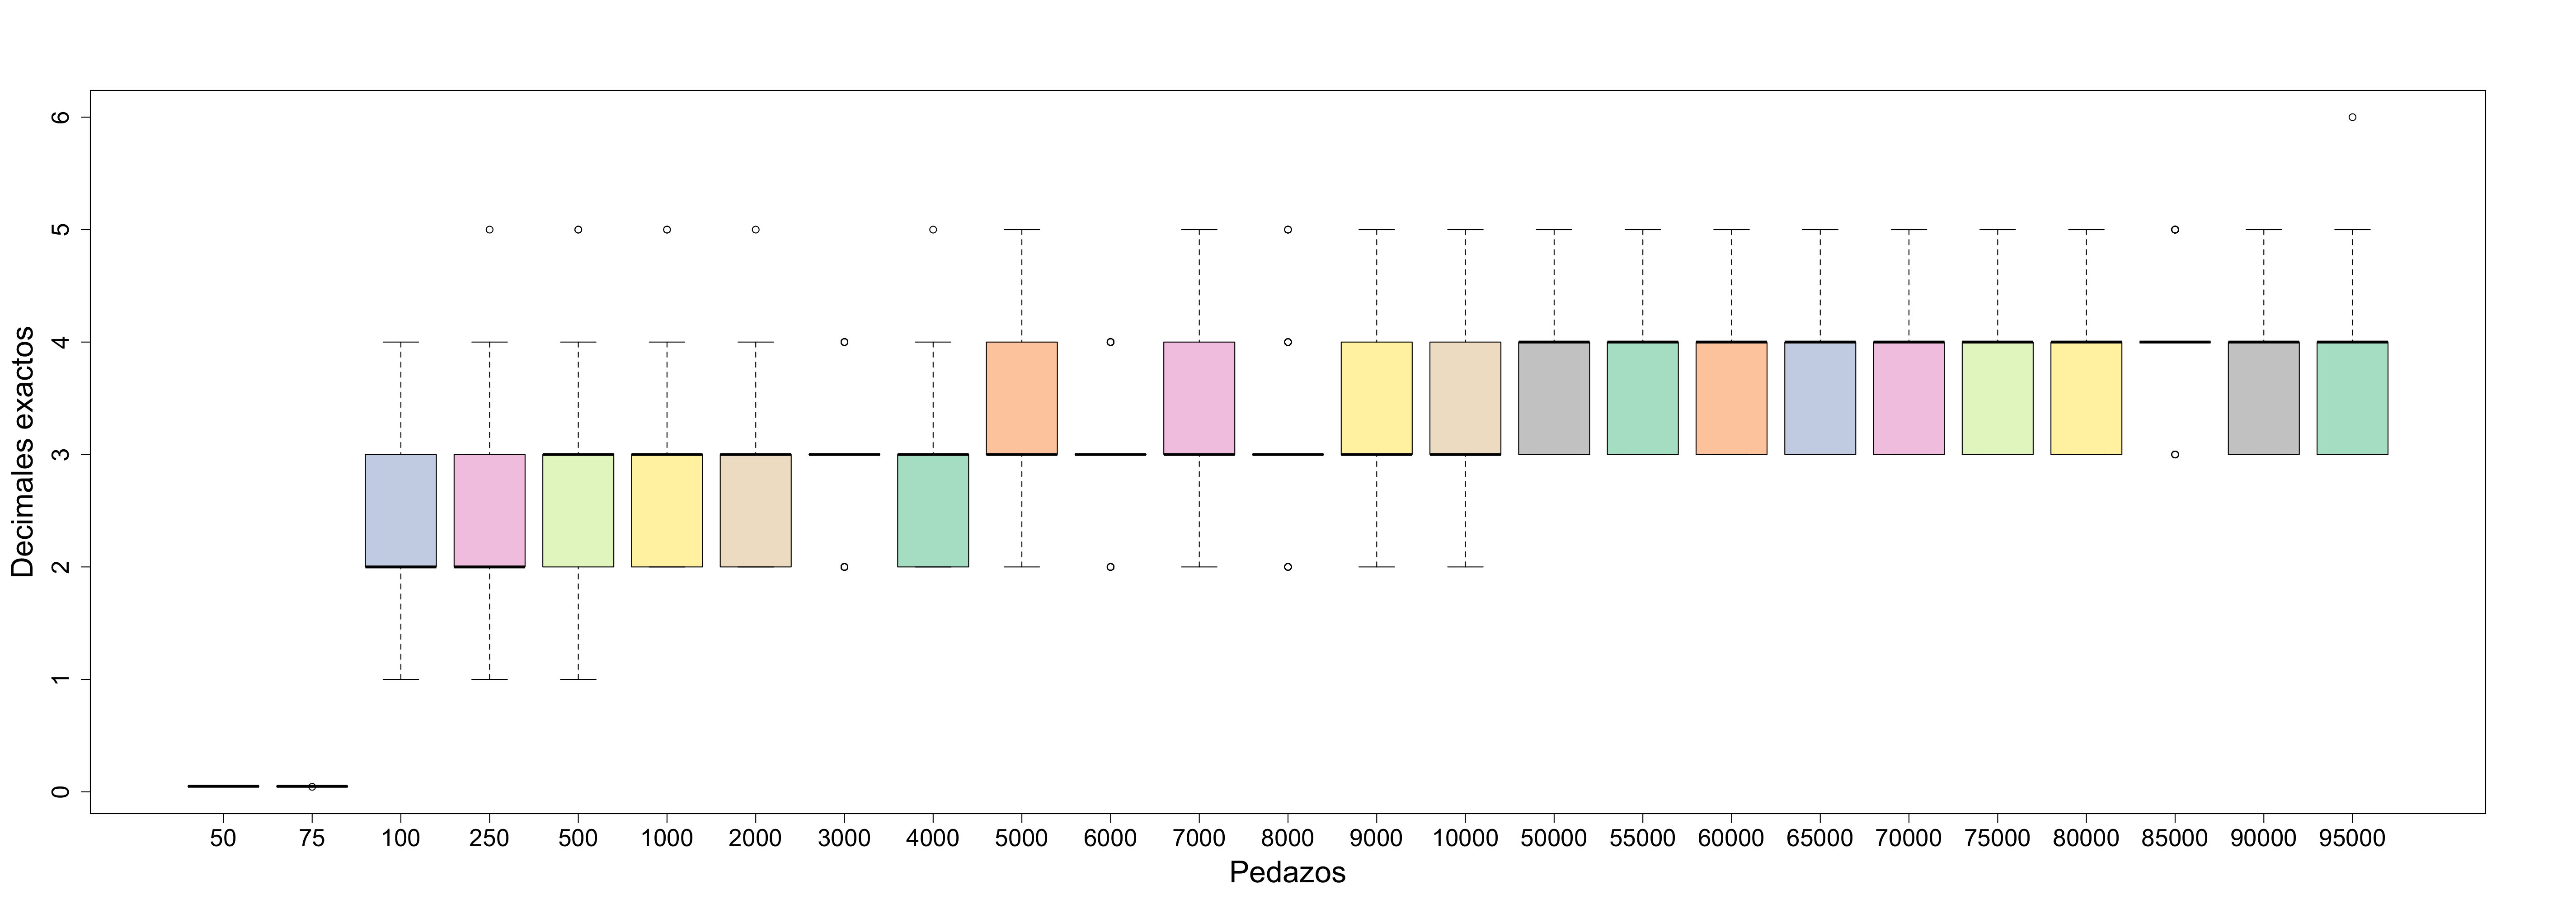
\includegraphics[width=\linewidth]{boxplot2.png}
	\caption{Gráficas de caja bigote de la cantidad de decimales en que coinciden los valores obtenidos de la integral con el valor de \texttt{wolfram}.}
	\label{box2}
\end{figure}
\subsection{Pruebas de correlación}
Se realiza la prueba de correlación para las columnas del tamaño de \texttt{pedazo} y la cantidad de decimales exactos. La prueba arroja un valor $p$ de $2.2\times 10^{-16}$ el cual es menor que 0.05, por lo que se rechaza la hipótesis nula y se concluye que hay correlación entre estas variables. Es decir, el tamaño de \texttt{pedazo} afecta a la cantidad de decimales exactos. En particular, se estima el coeficiente de correlación en 0.5576 por lo que se concluye que a mayor tamaño de \texttt{pedazo}, más decimales exactos hay.

\begin{verbatim}
	Pearson's product-moment correlation

data:  datos$Pedazo and datos$`Decimales Exactos`
t = 23.753, df = 1250, p-value < 2.2e-16
alternative hypothesis: true correlation is not equal to 0
95 percent confidence interval:
 0.5182761 0.5946934
sample estimates:
      cor 
0.5576652 
\end{verbatim}




\section{Reto 1}
Para el reto 1, hay que automatizar y paralelizar la estimación del valor $\pi$ de Kurt \cite{Kurt}. De manera similar que la tarea base, se varía el tamaño del parámetro \texttt{runs} en potencias de 10. En la figura \ref{box3} se aprecia que mientras es mayor el tamaño de \texttt{runs} más se aproxima al valor de \texttt{pi =} 3.141592 y en la figura \ref{box4} se muestran la cantidad de decimales a los que se aproxima. Aún aumentando a gran tamaño \texttt{runs}, no se pudo aproximar a más que cuatro decimales. 
\begin{figure}
	\centering
	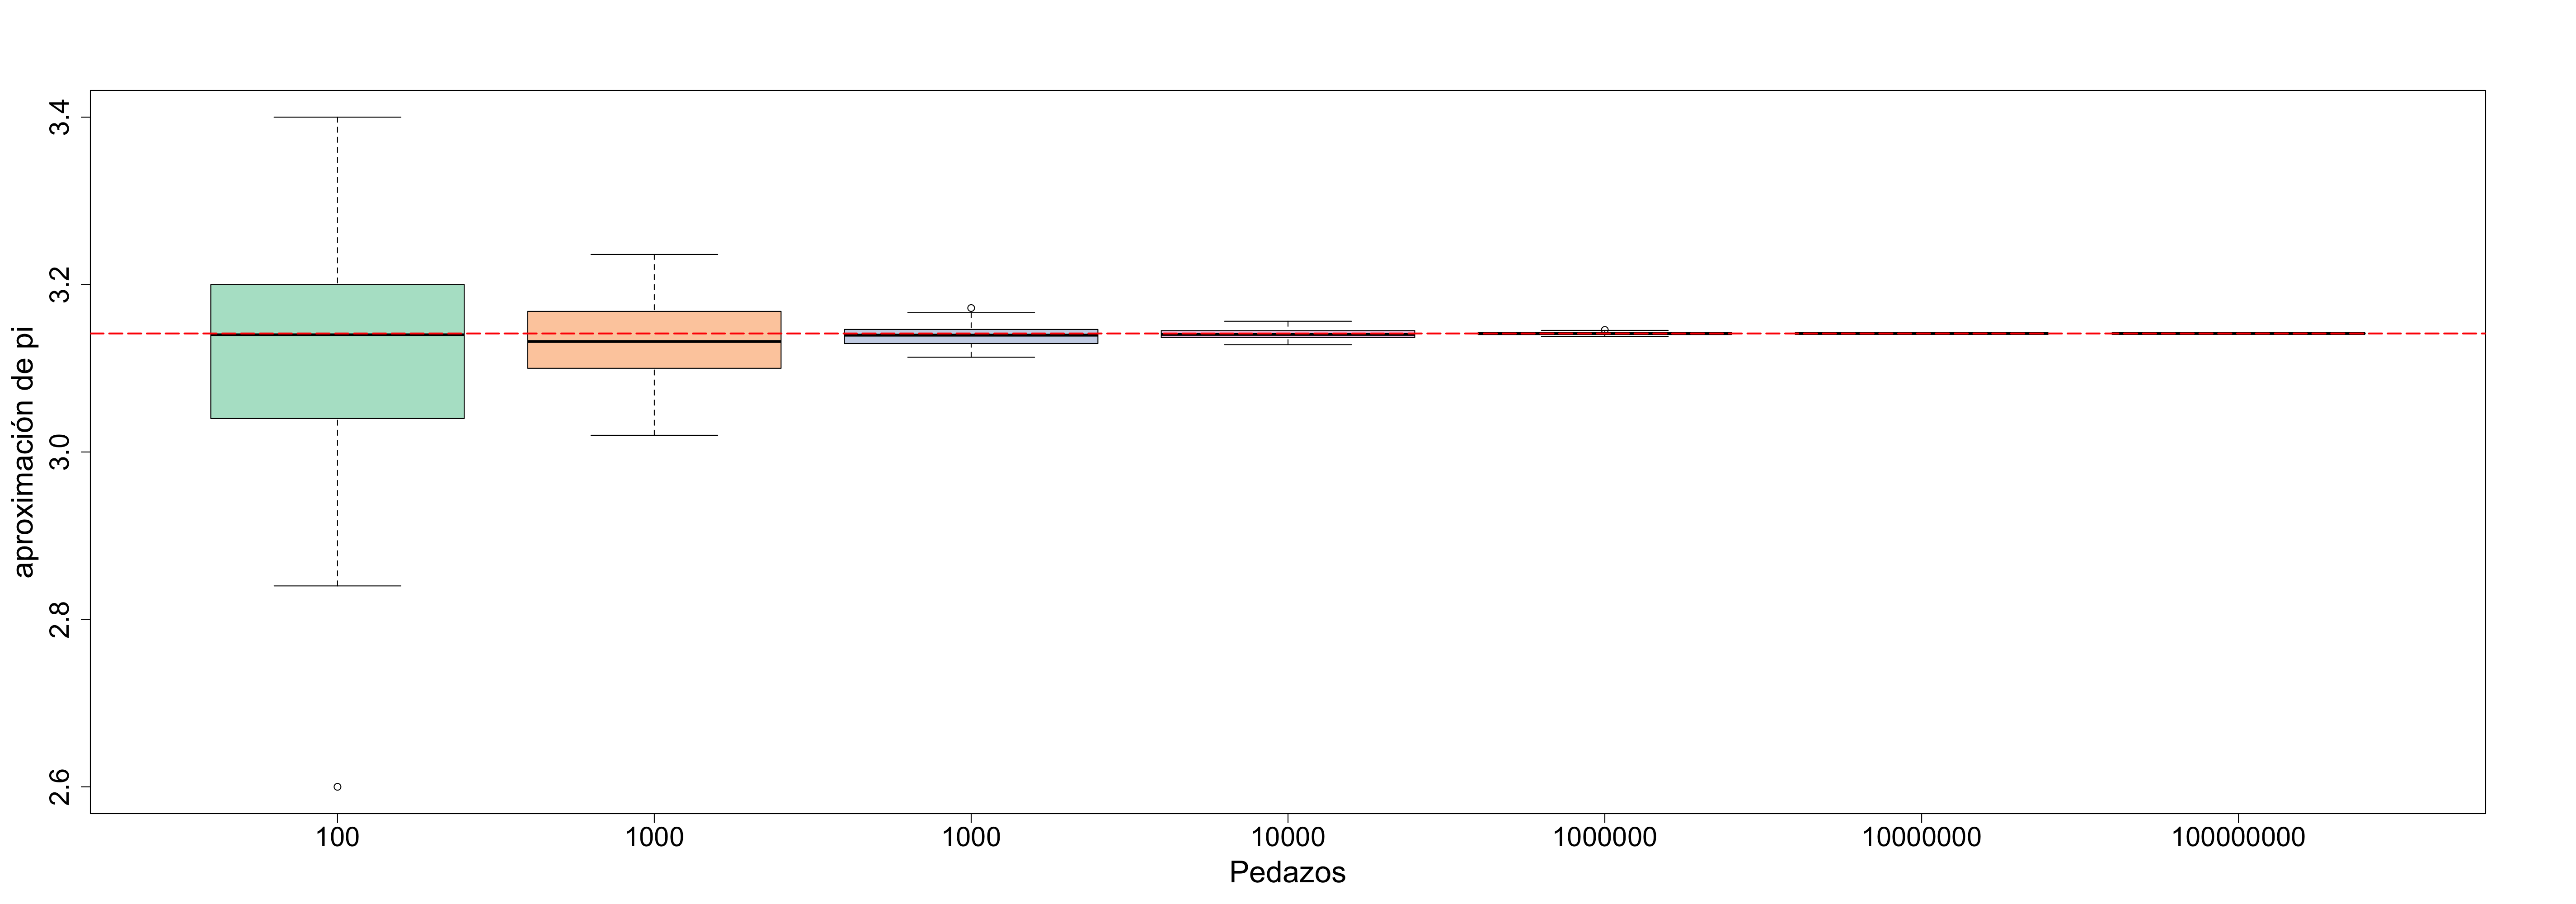
\includegraphics[width=\linewidth]{reto.png}
	\caption{Gráficas de caja bigote de las aproximaciones de \texttt{pi} obtenidas variando el tamaño de \texttt{runs}.}
	\label{box3}
\end{figure}

\begin{figure}
	\centering
	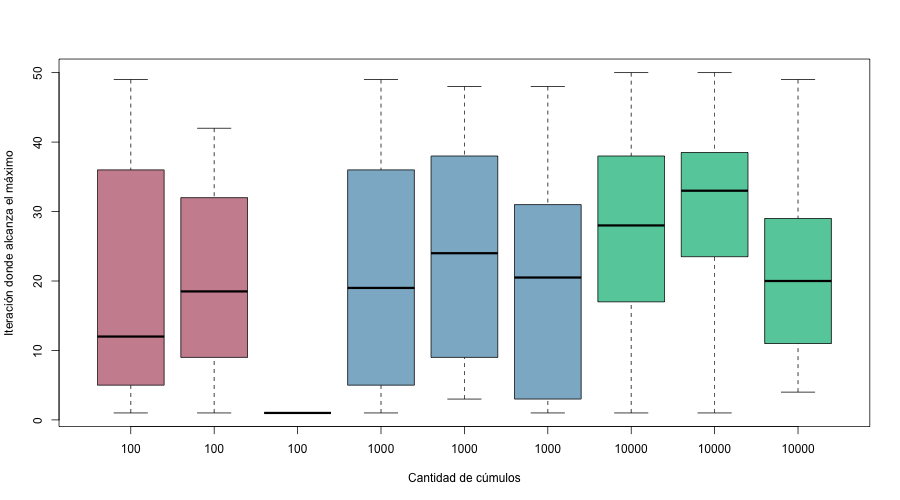
\includegraphics[width=\linewidth]{reto1.png}
	\caption{Gráficas de caja bigote de la cantidad de decimales que coincide la aproximación de $\pi$ obtenida con el valor de \texttt{pi}.}
	\label{box4}
\end{figure}
\bibliographystyle{plain} 
\bibliography{Referencias}


\end{document} 